\begin{figure}
    \centering
  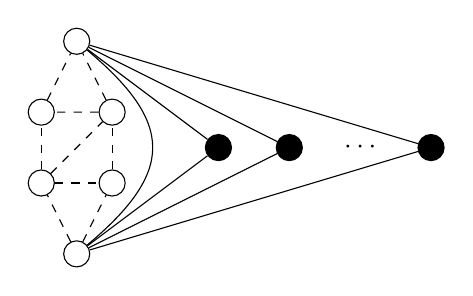
\begin{tikzpicture}[scale=0.9,rotate=90]
    \tikzstyle{w} = [circle, draw, fill=white,
    scale=1.0];
    \tikzstyle{b} = [circle, draw, fill=black,
    scale=1.0];
    \tikzstyle{gd} = [black,dashed,-];

    \node[w] (1) at (0,0){};
    \node[w] (2) at (1,0.5){};
    \node[w] (3) at (1,-0.5){};
    \node[w] (4) at (2,0.5){};
    \node[w] (5) at (2,-0.5){};
    \node[w] (6) at (3,0){};

    \node[b] (7) at (1.5,-2){};
    \node[b] (8) at (1.5,-3){};
    \node[] (9) at (1.5,-4){$\cdots$};
    \node[b] (9) at (1.5,-5){};

    \path[gd] (1) edge (2)
                  edge (3)
              (2) edge (3)
                  edge (4)
                  edge (5)
              (3) edge (5)
              (4) edge (6)
              (5) edge (6)
                  edge (4);
                  
    \path[-]  (1) edge [bend right=50,
                        looseness = 1.5] (6);
    \path[-]  (7) edge (1)
                  edge (6)
              (8) edge (1)
                  edge (6)
              (9) edge (1)
                  edge (6);
                  


  \end{tikzpicture}
    \caption{A problematic graph for algorithm 
    that stores only nodes CPM0.
    It merges dashed and black triangle 
    communities if any 
    black clique is considered after 
    all cliques of the dashed community.
    The number of black cliques
    can be arbitrary large, 
    implying that CPM0 with 
    a random order of clique 
    processing will almost surely merge two 
    communities when the number of black cliques
    tends to infinity.
    Our approximate
    Algorithms~\ref{algo:ckcom2}
    and~\ref{algo:ckcom3} 
    stores links not just nodes. 
    They are immune to this problematic case.
    }
    \label{gr0}
\end{figure}